%%%%%%%%%%%%%%%%%%%%%%%%%%%%%%%%%%%%%%%%%%%%%%%%%%%%%%%%%%%%%%%%%%%%%%%%%%%%%%%%
%2345678901234567890123456789012345678901234567890123456789012345678901234567890
%        1         2         3         4         5         6         7         8

\documentclass[letterpaper, 10pt, conference]{ieeeconf}                             
\IEEEoverridecommandlockouts         % Needed if you want to use the \thanks command
                                                     
\overrideIEEEmargins                                                            


\usepackage{times} % assumes new font selection scheme installed
\usepackage{amsmath}
\usepackage{amssymb,longtable,calc}
\usepackage{mathptmx}
\usepackage[T1]{fontenc}                                                        
\usepackage[utf8]{inputenc}                                                     
\usepackage[english]{babel}                                                     
\usepackage{epsfig}                                                             
\usepackage{subfigure}                                                          
\usepackage{textcomp} %<- allows to use \textdegree but may overwrite           
                      %other settings                                           
\usepackage[textwidth=2cm,colorinlistoftodos,disable]{todonotes} %add disable   
     
										                         
\usepackage{tikz}                                                               
\usetikzlibrary{arrows,positioning,fit,shapes,calc}
\usetikzlibrary{matrix}
\usepackage{flushend}                                                           
\usepackage{hyperref}  
\usepackage{amsmath}                                                         
% \usepackage{multirow}   
\usepackage{dirtytalk}% for \say

\usepackage{algorithm}    
\usepackage{algorithmic}

\usepackage{pgfplots} 
\usepackage{pgfplotstable}

\usepackage{cite}

% helper packages to work on the draft
\usepackage[tikz]{bclogo}
\usepackage{lipsum}

\usepackage{standalone}

\pgfplotsset{compat=newest}
\pgfplotsset{ 
  tick label style={font=\footnotesize}, 
  label style={font=\footnotesize}, 
  legend style={font=\footnotesize},
  title style = {font=\small}
}
\pgfplotscreateplotcyclelist{line style}{% 
  solid, mark options = {scale = .75}, every mark/.append style={fill=gray},mark=*\\% 
  densely dashed,mark options = {scale = .75},every mark/.append style={solid,fill=gray},mark=*\\% 
  densely dotted,mark options = {scale = .75},every mark/.append style={solid,fill=gray},mark=*\\% 
  dashed,mark options = {scale = .75},every mark/.append style={solid,fill=gray},mark=*\\% 
  dotted,mark options = {scale = .75},every mark/.append style={solid,fill=gray},mark=*\\% 
}
\pgfplotscreateplotcyclelist{bar style}{% 
  solid, fill=black!60!white\\%
  solid, fill=black!45!white\\%
  solid, fill=black!35!white\\%
  solid, fill=black!25!white\\%
}


\usepackage{xspace}
\makeatletter                                                                   
\DeclareTextCommandDefault{\textregisteredalt}{\footnotesize\textcircled{%      
      \check@mathfonts\fontsize\sf@size\z@\math@fontsfalse\selectfont R}}       
\DeclareRobustCommand\onedot{\futurelet\@let@token\@onedot}                     
\def\@onedot{\ifx\@let@token.\else.\null\fi\xspace}                             
\def\eg{e.g\onedot}                                                             
\def\ie{i.e\onedot}                                                             
\def\vgl{see }                                                                  
\def\Fig{Fig\onedot }                                                           
\def\Tab{Tab\onedot }                                                           
\def\Eq{Eq\onedot }
\def\Sec{Sec\onedot}                                                            
\def\etc{etc\onedot}                                                            
\def\etal{\textsl{et al}\onedot}                                                
\def\argmin{\mathop{\rm arg\,min}}                                              
\makeatother
                                                                    
\definecolor{lightGray}{rgb}{0.0,0.0,0.0}
                                                                                
\title{\LARGE \bf Team CVAP's Picking System at the Amazon Picking Challenge 2015}                                                                               
                                                                                
                                                                                
\author{Kaiyu Hang ~~ Francisco E. Vi\~na B. ~~ Michele Colledanchise \\ ~~ Karl Pauwels ~~ Alessandro Pieropan ~~ Danica Kragic%
\thanks{All team members contributed equally in this work.}%
\thanks{K. Hang, F. E. Vi\~na B., M. Colledanchise, K. Pauwels, A. Pieropan and D. Kragic are with the
Robotics, Perception and Learning Lab (RPL), CAS, CSC at KTH Royal Institute of
Technology, Stockholm, Sweden.}%
}

\begin{document}                                                                
                                                                                
\maketitle                                                                      
\thispagestyle{empty}                                                           
\pagestyle{empty}



%%%%%%%%%%%%%%%%%%%%%%%%%%%%%% ABSTRACT %%%%%%%%%%%%%%%%%%%%%%%%%%%%%%%%%%%%%
\begin{abstract}

In this paper we will present our framework used in the Amazon Picking Challenge in 2015 and some of the  lessons learned that may prove useful to researchers and future teams participating in the competition. The competition proved to be a very useful occasion to integrate the work of various researchers at the Robotics, Perception and Learning laboratory of KTH, measure the performance of our robotics system and define the future direction of our research.

\end{abstract}

%%%%%%%%%%%%%%%%%%%%%%%%%%%%%% INTRODUCTION %%%%%%%%%%%%%%%%%%%%%%%%%%%%%%%%%%%
% \begin{}
\section{INTRODUCTION}
\label{sec:introduction}

There are three main criteria engineers evaluate when determining the need of robots in certain applications: dirty, dull and dangerous. Those are known as the 3D of Robotics. The application proposed by the Amazon Picking Challenge meets certainly the second criteria as picking and placing objects in boxes is a very repetitive and dull task with tremendous potential
for automation. However, despite the defined and controlled environment the application of robots is still very challenging due to the nature of the objects to handle.
In this work we present the framework we developed at the Robotic, Perception and Learning lab (RPL) in 2015 with the purpose of sharing the lessons learned with the community.
First we will describe the platform used in the competition in Sec.\ref{sec:platform} to motivate the strategy we adopted in Sec.\ref{sec:strategy}. Then we will describe the core of our system that controls the whole pipeline of actions using Behavior Trees (BTs) in Sec.\ref{sec:trees}. Then we will describe our perception module starting with the localization of the shelf in Sec.\ref{sec:shelf} and detections of the objects \ref{sec:vision}. Finally we will describe our grasping strategy in Sec.~\ref{sec:grasping} and draw some conclusion about the limitations of our system in Sec.\ref{sec:conclusion}.

%% %%%%%%%%%%%%%%%%%%%%%%%%%%% PR2 %%%%%%%%%%%%%%%%%%%%%%%%%%%%%%%% 
\section{Platform}
\label{sec:platform}

We used the PR2 research robot from Willow Garage shown in Fig.
\ref{fig:PR2} for the 2015 APC competition. The robot consists of two
7-DOF manipulators attached to a height-adjustable torso and equipped with parallel-jaw
grippers. A pan-tilt controllable robot head is located on the upper part of the robot
and equipped with a set of RGB cameras and a Kinect camera which we used in
our object segmentation system. The robot is also
equipped with a tilt-controllable laser scanner located right beneath the head which we
also used for object segmentation purposes.
A set of 4 wheels at the base provides the robot with omnidirectional mobility, which we
exploited in order to control the robot back and forth from the shelf to pick up objects
and release them in the target box.


\begin{figure}[h]
\centering
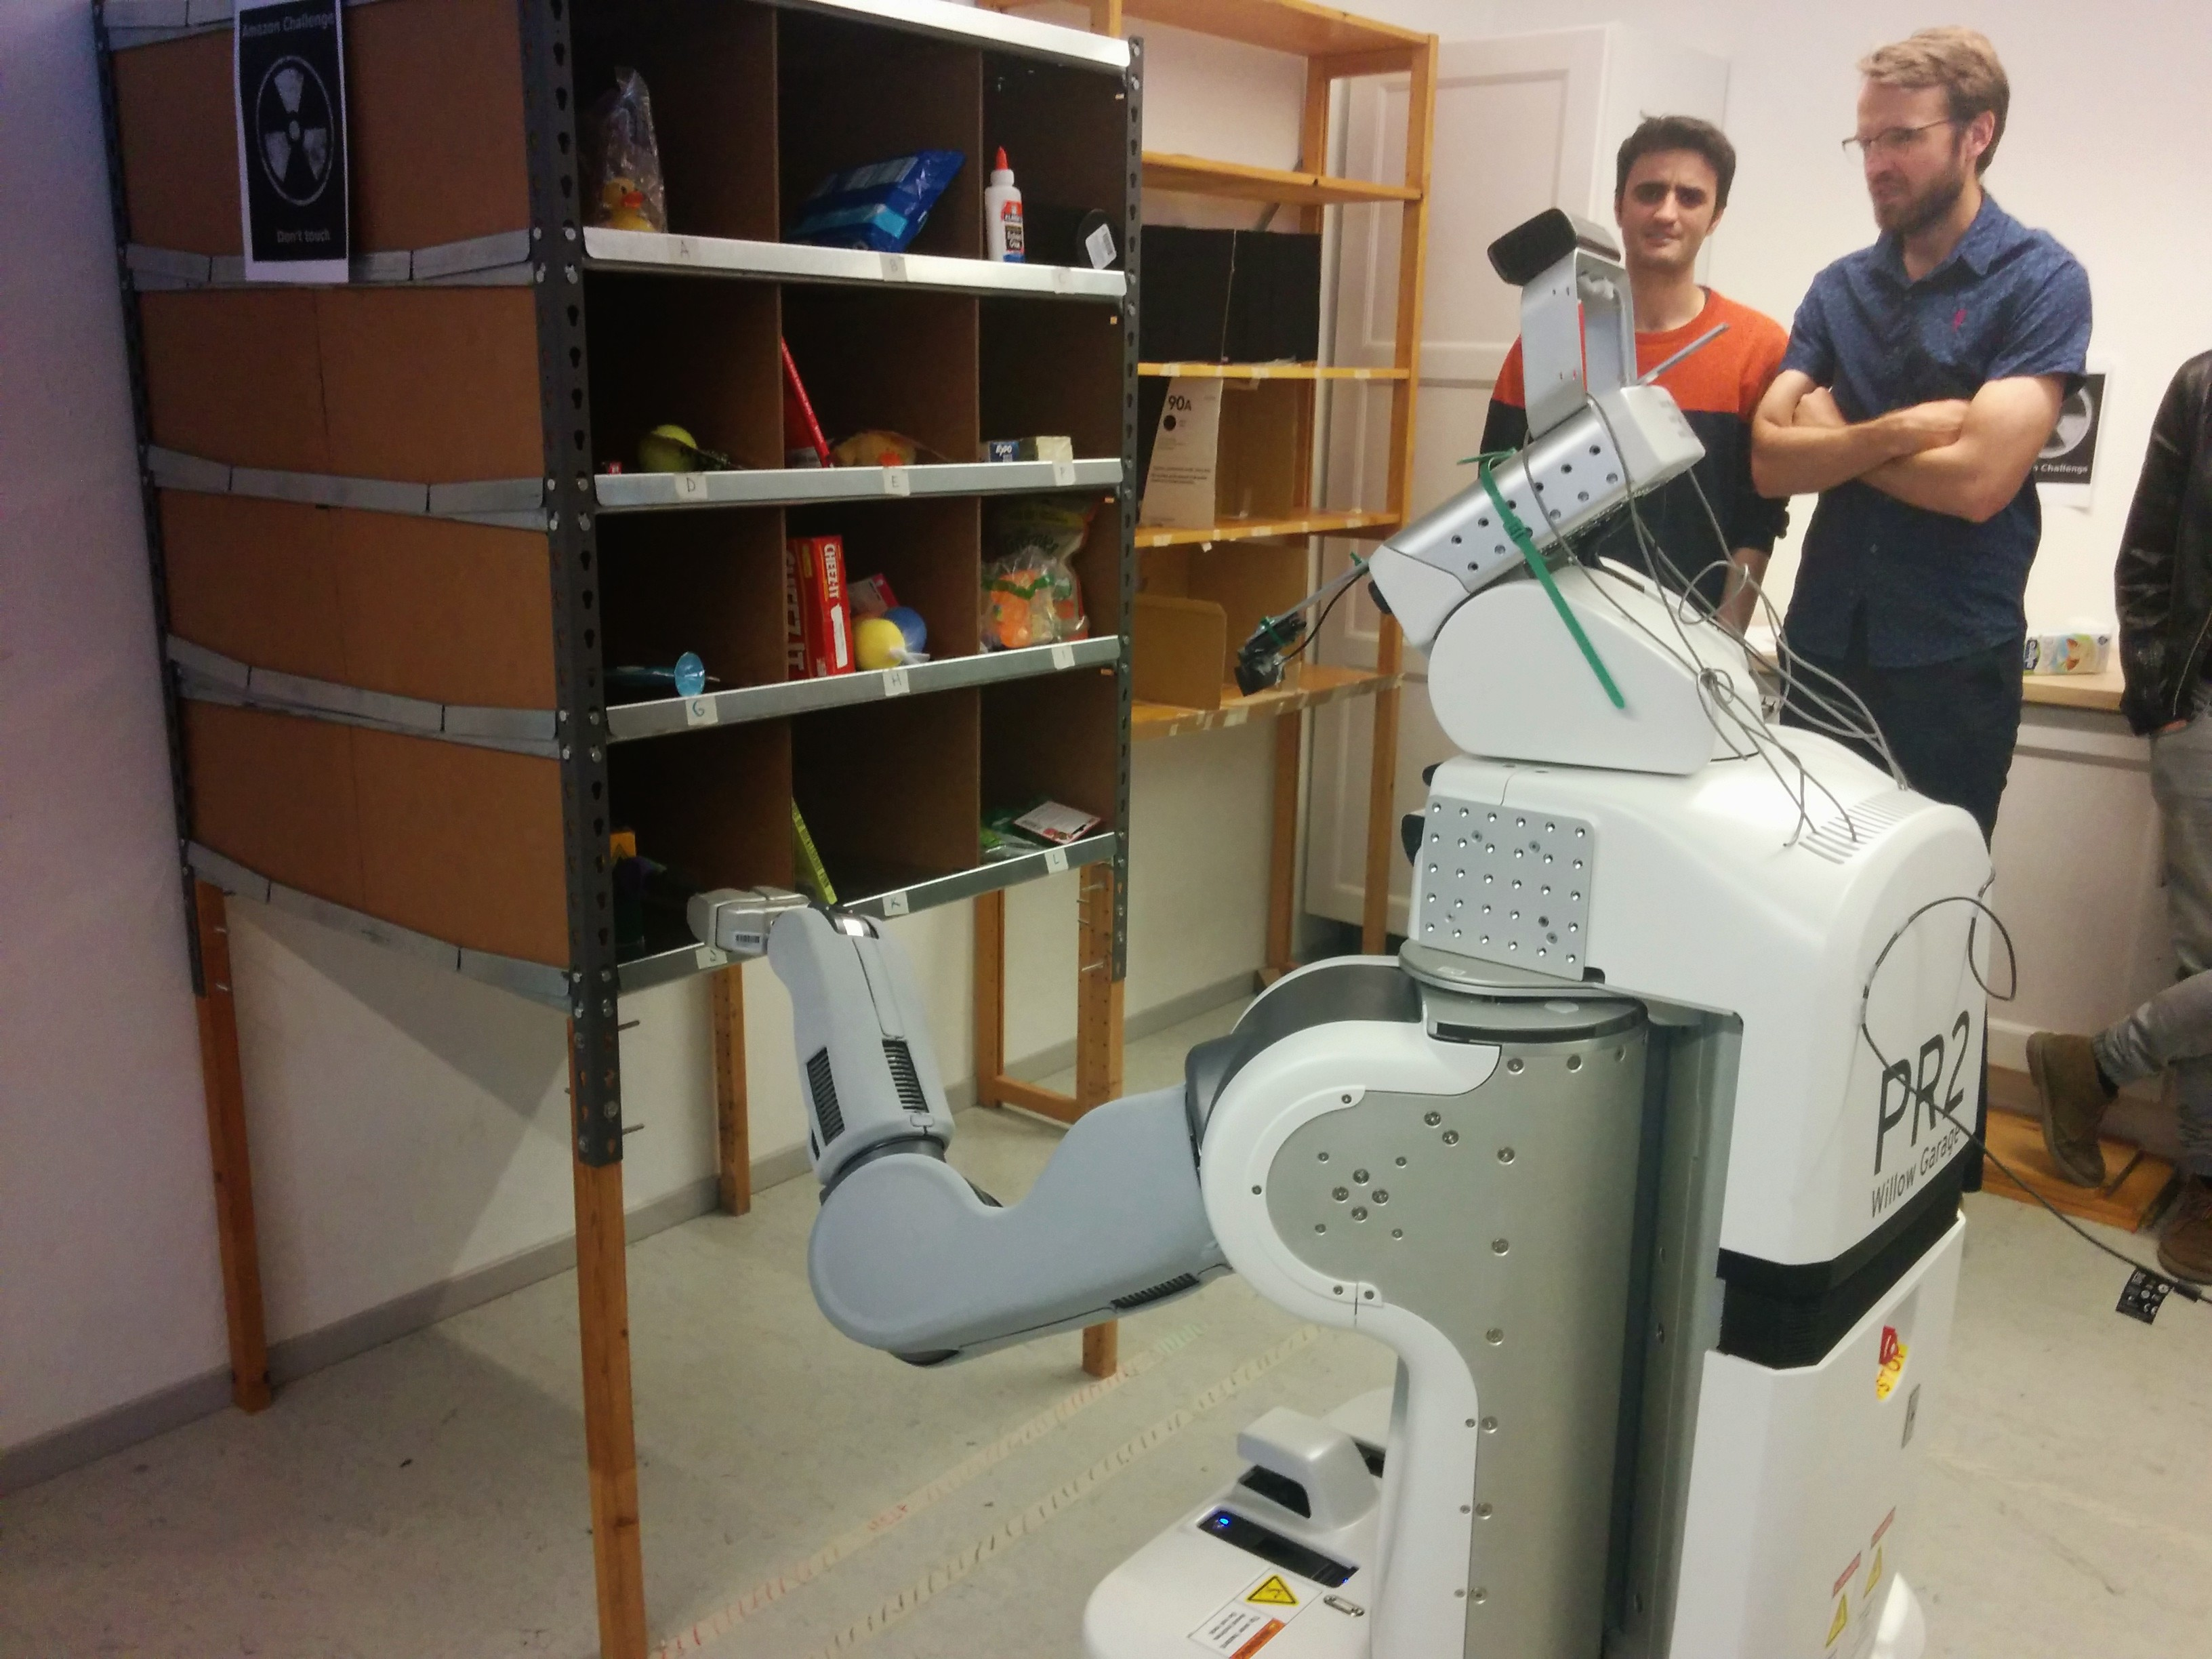
\includegraphics[trim=15.0cm 4.0cm 6.0cm 0cm,clip=true,scale=0.07]{figures/pr2.jpg}
\caption{Team CVAP's PR2 robot platform used for the Amazon Picking Challenge 2015 in Seattle, USA.}\label{fig:baxter}
\end{figure}

We provided some minor hardware modifications to the PR2 robot in order to
address some of the challenges  of the picking task,
namely custom-made extension fingers for the parallel gripper in order
to be able to reach further inside of the bins of the shelf and a high resolution
webcamera which we attached on the PR2's head in order to get
a richer set of image features for our Simtrack vision system to detect the target 
objets in the shelf.

The robot ran on an Ubuntu 12.04 computer with a real-time linux kernel that provides
1 KHz manipulator control. All the high level task execution, perception, grasping and manipulation software components were developed under the Robot Operating System (ROS).


%% %%%%%%%%%%%%%%%%%%%%%%%%%%% PR2 %%%%%%%%%%%%%%%%%%%%%%%%%%%%%%%% 
\section{Strategy}
\label{sec:strategy}

In 2015 the competition consisted in picking one object from each of the 12 bins of the shelf within 20 minutes. Each bin could contain from one up to four objects making the recognition and grasping of objects increasingly difficult. In order to design our strategy we had three main limitations to consider. First the PR2 could not reach the highest level of the shelf where three bin were located. Second two of the objects of the competition were bigger than the maximum aperture of the PR2 gripper. Third, it takes the PR2 about 30 seconds to raise the torso from the lowest position to the highest. Given the time requirements that operation resulted very expensive. Therefore our strategy consisted in starting from the lowest level of the shelf giving priority to the bins with one or two objects. Once the bins were cleared the PR2 would raise the torso to address the next level of the shelf. The more complex bins with multiple objects were left at the end disregarding the level they were located. Given the limitation of our robot, the known structure of shelf and the object to grasp our framework would decide what grasp strategy to apply from a pre-defined set.

%% %%%%%%%%%%%%%%%%%%%%%%%%%%% BTS %%%%%%%%%%%%%%%%%%%%%%%%%%%%%%%%
\section{Behavior Trees}
\label{sec:trees}


BTs are a graphical mathematical model for reactive fault tolerant action executions. They were introduced in the video-game industry to control non-player characters, and they are now an established tool appearing in textbooks \cite{millington2009artificial,rabin2014gameAiPro} and generic game-coding software such as Pygame1, Craft AI 2, and the Unreal Engine3. In robotics, BTs are appreciated for being highly modular, flexible and reusable, and have also been shown to generalize other successful control architectures such as the Subsumption architecture, Decision Trees~\cite{colledachise17tro} and the Teleo-reactive Paradigm~\cite{Colledanchise16iros}.
%\subsection{Semantic}
%Here we breafly describe the semantic of BTs. An exaustive description can be found in~\cite{colledachise17tro}.
% 
%A BT is a directed rooted tree with the the common definition of \emph{parent} and \emph{child} node. Graphically, the children of nodes are placed below it. The children nodes are executed in the order from left to right.
%
%The execution of a BT begins from the root node that sends \emph{ticks}~\footnote{A tick is a signal that allows the execution of a node} with a given frequency to its (only) child. When a parent sends a tick to a child, the execution of this is allowed. The child returns to the parent a status \emph{running} if its execution has not finished yet, \emph{success} if it has achieved its goal, or \emph{failure} otherwise.\\ 
%There are four types of internal nodes (fallback, sequence, parallel, and decorator) and two types of leaf nodes (action and condition). Below we describe the execution of the nodes used in our framework.
%
%\paragraph*{Fallback}
%The fallback node send ticks to its children from the  left, returning success (running) when it finds a child that returns success (running). It returns failure only when all the children return failure. When a child returns running or success, the fallback node does not send ticks the next child (if any).
%A fallback node is graphically represented by a box labeled with a \say{?}, as in Figure~\ref{bg.fig.sel}.
%
%\paragraph*{Sequence}
%The sequence node sends ticks to its children from the  left, returning failure (running) when it finds a child that returns failure (running). It returns success only when all the children return success. When a child returns running or failure, the sequence node does not send ticks the next child (if any). A sequence node is graphically represented by a box labeled with a \say{$\rightarrow$}, as in Figure~\ref{bg.fig.seq}.
%
%\paragraph*{Action}
%The action node performs an action. It return running while the action is being performed. It return success of the action is completed correctly, otherwise it return failure. An action node is graphically represented by a rectangle labeled with the name of the action, as in Figure~\ref{bg.fig.seq}.
%
%
%\paragraph*{Condition}
%The condition node checks if a condition is satisfied or not, returning success or failure accordingly.  An action node is graphically represented by an ellipse labeled with the name of the condition, as in Figure~\ref{bg.fig.seq}.
%
%
%\subsection{BTs in APC}
In our framework, the use of BTs allowed us to have a control architecture that is:

\begin{itemize}
\item \textbf{Reactive:} The Reactive execution allowed us to have a system that rapidly reacts to unexpected changes. For example, if an object slips out of the robot gripper, the robot will automatically stop and pick it up again without the need to re-plan or change the BT; or if the position of a robot is lost, the robot will re-execute the routine of the object detection.
\item \textbf{Modular:} The Modular design allowed us to subdivide the behavior into smaller modules, that were independently created and then used in different stages of the project. This design allowed our heterogeneity developers’ expertise, letting developers implementing their code in their preferred programming language and style.
\item \textbf{Fault Tolerant:} The fault tolerant allowed us to handle actions failure by composing different actions meant for the same goals in a fallback. (e.g. different types of grasps).
\end{itemize}





%% %%%%%%%%%%%%%%%%%%%%%%%%%%% SHELF %%%%%%%%%%%%%%%%%%%%%%%%%%%%%%%% 
\section{Shelf Localization and Base Movement}
\label{sec:shelf}

As described in Sec.~\ref{sec:platform}, we used a PR2 as our robot platform. Since the arms' reachability of PR2 is relatively small in comparison to the shelf size, it is not feasible to define a fixed location for the robot to achieve the required task. As such, we have to exploit the mobility to enlarge the working space, so that the robot would be able to reach and grasp from most of the shelf bins, as well as loading the grasped objects into the order bin.

For this, shelf localization, which serves as the only landmark in the workcell, is essential for our system to guide the robot navigating between different grasping positions. Since the robot movement accumulates localization errors, it is necessary to localize the shelf in real time to close the control loop for base movement. 

\begin{figure}[htb]
\centering
	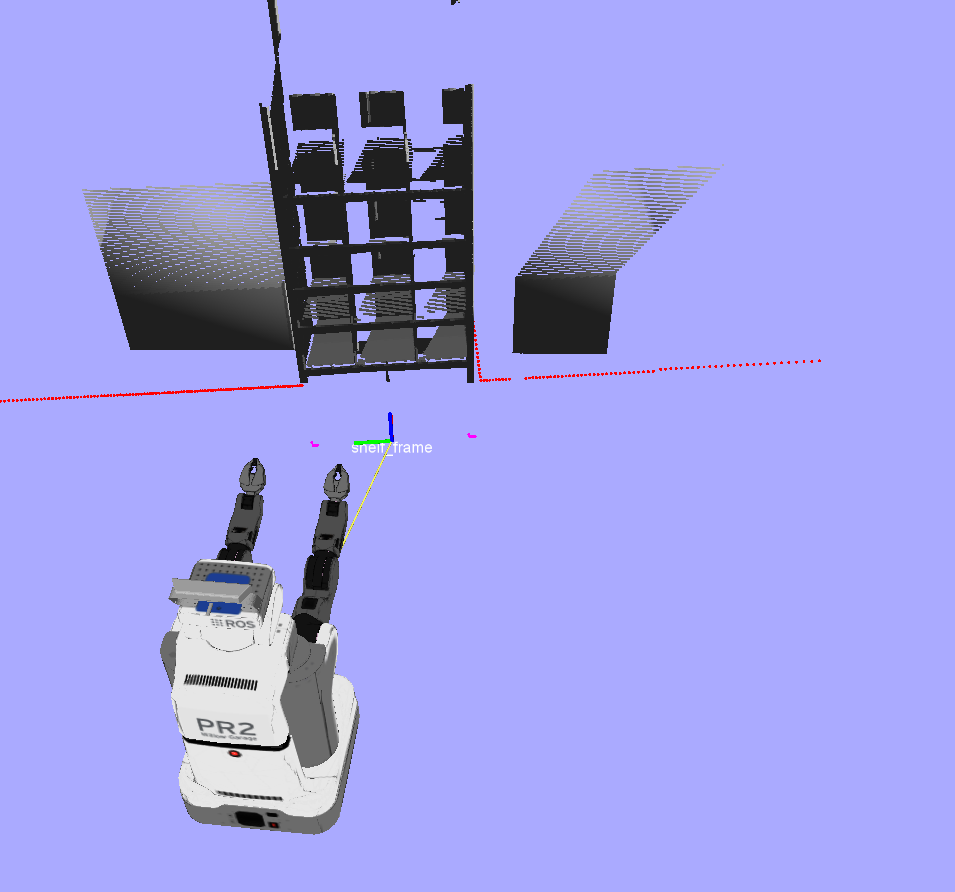
\includegraphics[height=0.39\columnwidth]{figures/localization.png}
	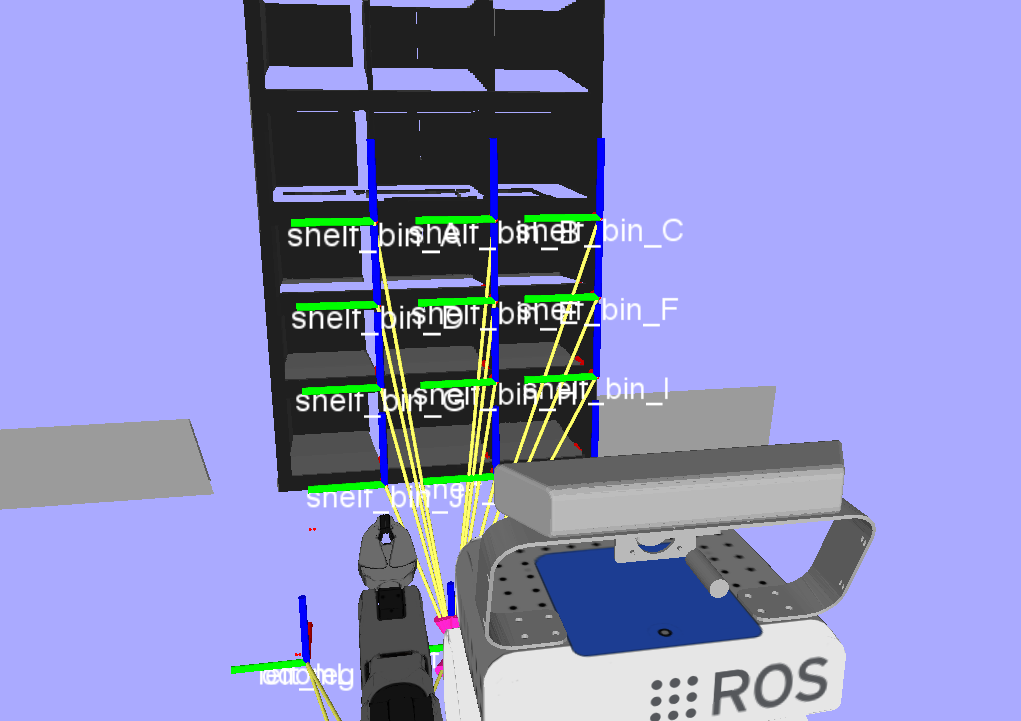
\includegraphics[height=0.39\columnwidth]{figures/binFrames.png}
        \caption{\emph{Left}: An example of shelf localization shown in rviz. The x and y coordinates of shelf\_frame is defined as the center of two front legs, while the height of it is the same as the base\_laser\_link. \emph{Right}: The bin frames are located at the right bottom corner of each bin.}
        \label{fig:localization}
\end{figure}

As shown in Fig.~\ref{fig:localization}, we use the base laser scanner to localize the two front legs of the shelf. Observing that the shelf is located in front of the robot, where no any other objects are close by. Therefore, it is reasonable to find the closest point cluster and consider it as one of the legs, while the remaining cluster is considered as another leg. However, this is not a reliable procedure as there could be noise or other unexpected objects, e.g., human legs. As such, our shelf localization consists of two procedures as follows:

\begin{itemize}
 \item \textbf{Detection:} Once the front legs are detected, before the system starts to autonomously work on assigned tasks, a human supervisor needs to confirm to the robot that the detection is correct. In case when the detection is incorrect, we need to clear the occlusions in front of the shelf until a confirmation is made.
 \item \textbf{Tracking:} While the robot is moving, given that we know the motion model of the robot, we update the shelf localization using a Kalman filter.
\end{itemize}

Having localized the shelf, we further estimate the shelf bin frames based on the known mesh model, see Fig.~\ref{fig:localization}. As will be described in Sec.~\ref{sec:grasping}, knowing the bin frames will facilitate the grasp planning in our system.

%% %%%%%%%%%%%%%%%%%%%%%%%%%%% VISION %%%%%%%%%%%%%%%%%%%%%%%%%%%%%%%%
\section{Vision}
\label{sec:vision}

\subsection{Simtrack}

We created high-quality 3D textured models from all objects provided for the challenge using the approach described in~\cite{pokorny_2017}. To summarize briefly, each object is placed on a textured background consisting of a collection of newspapers and approximately 40 pictures are taken from various angles. The object is then constructed using Autodesk123D catch services~\cite{autodesk} and postprocessed to separate it from the background, remove holes, reduce the mesh resolution, etc. For the texture-based detection discussed next, we also extracted SIFT-keypoints~\cite{lowe04} from images synthesized by rendering the model from multiple viewpoints. The final object models were used for detection and grasp planning.

A large proportion of the challenge objects contained sufficient texture for keypoint-based pose detection. When such objects were present in the bin, we relied on a texture-based pose estimation method. We used high resolution images obtained from a Logitech~C920 webcam mounted on the robot head. We processed a central 1152$\times$768 pixel region of the full 2304$\times$1536 input image for object detection. The robot head was always oriented towards the bin under consideration so that this region of interest was guaranteed to contain the objects. Our object pose detection framework, SimTrack, first extracts SIFT-features from the image and matches these to the database of SIFT features extracted from the object models in the modeling stage. In the detection stage, the objects are identified, and a rough initial pose is obtained. This pose is then iteratively refined by rendering the textured object models at the current pose  estimate, and locally matching their appearance to the observed image~\cite{pauwels_simtrack_2015}. SimTrack uses a phase-based optical flow algorithm in this refinement (or tracking) stage to reduce sensitivity to intensity differences between model and observed image. SimTrack exploits the rich appearance and shape information of the models and correctly handles occlusions within and between objects. SimTrack is publicly available as a ROS module~\cite{simtrack_github}.


\subsection{Volumetric Reasoning}

We designed a fallback strategy based on 3D point cloud volumetric reasoning in case our system could not recognize the objects using SimTrack. Knowing the location of the shelf and the bins, as shown in Fig.~\ref{fig:localization}, we use the PR2 tilting laser scanner mounted on the torso to build an accurate point cloud within the target bin. We use the 3D model of the shelf and its estimated location to remove any point belonging to the shelf from the constructed point cloud to obtain a cloud of the inside of a bin. Then, we  apply euclidean clustering to generate plausible object hypothesis. Given that the number of objects in the bin is known, we apply our clustering strategy iteratively, increasing the distance threshold, in order to obtain as many clusters as the expected number of objects. Once the clusters are found we formulate the problem of finding the right object to pick as a bipartite graph matching problem where the nodes on one side are the found clusters characterized by their volumes and the nodes on the other side are the 3D models of the expected objects and their corresponding volumes.

%% %%%%%%%%%%%%%%%%%%%%%%%%%%% GRASPING %%%%%%%%%%%%%%%%%%%%%%%%%%%%%%%%
\section{Manipulation and Grasping}
\label{sec:grasping}

For robot arm motion planning we used the MoveIt! software framework and its
default randomized motion planners. Even though MoveIt! provides seamless integration with ROS-enabled robots, we faced some difficulties when applying it in our PR2 APC setup. The randomized planners (e.g. RRT) often had difficulties in finding collision free trajectories
to move the robot arm in constrained spaces such as the interior of the bins. Even when it did find suitable trajectories, they would often  generate very large joint displacements even for small end-effector cartesian motions, which 
increased the chance of generating collisions with the shelf. 
We partially alleviated these
problems by exploiting the simpler 2D kinematic motion control of the robot base e.g.
to retreat from the shelf. Optimization based motion planners and a more specialized
kinematic structure of the robot are possible directions of work that would address
these issues. 

Once the target object is detected, the object frame is obtained from our vision system. Given that the PR2 is equipped with parallel grippers, we must then decide from which position and in which direction the gripper is going to approach the object in order to then grasp the object
in a secure way. For this, we always project the object frame based on the bin frame such that the X axis of the object frame points inwards the shelf, and the Z axis points downwards. Note that in order to ensure that the object can be approached without generating collisions,
we manually labeled all objects offline so that the X axis returned from the vision system can always be approached with the gripper, i.e. that the gripper opening is wide enough to grasp the corresponding side of the object. Thereafter, similarly to the grasping stages in \cite{hang2016b}, our grasping system works in the following steps:
\begin{itemize}
 \item \textbf{Pre-grasping:} The gripper is posed in front of the bin and aligned in X axis of object frame, the gripper's opening direction is aligned in the XY plane of object frame.
 \item \textbf{Approaching:} The gripper approaches the object in X direction until a pre-determined depth in the object frame is reached.
 \item \textbf{Grasping and lifting:} The gripper closes and lifts the object to a pre-determined height. At this point, we read the gripper's joint angle to check whether the object is grasped. If not, the system will return failure and give control back to the behavior tree. Otherwise, it returns success and continue to the next step.
 \item \textbf{Post-grasping:} When the object is grasped, it is not trivial to plan a motion to move the arm out of the shelf, especially for large objects. Therefore, we first move the object to the bin center, and then move the whole robot backwards. Once the object is out of the shelf, the robot goes to the order bin and puts the object into it.
\end{itemize}
In cases when the target object is very small, e.g., tennis ball and duck toy etc., the approaching procedure shown above is not able to reach the object due to the collision with the bin bottom. In those cases, our system will first try to approach the above area of the object, and then move downwards to reach the desired grasping pose. It is worthwhile noticing that, dividing the grasping motion into steps significantly increased the success rate for MoveIt! to find solutions within a short time limitation, since the above steps efficiently guides the motion planner through narrow passages posed by the small bin areas. 


\section{Conclusion}
\label{sec:conclusion}

We presented the framework used in the APC 2015 and the challenges that we faced.
Overall, perception was the most challenging component for the competition although
the challenges inherent to manipulation and grasping should not be underestimated. We can propose
the following suggestions to researchers and engineers designing bin-picking robotic
systems given our experience at the APC 2015:

\begin{itemize}
\item \textbf{Robot kinematic design.} In order to facilitate motion control of the robot manipulator   and minimize the risk of generating collisions it is best to design its kinematic
  structure to be completely tailored to the task instead of a general purpose humanoid kinematic configuration such as our PR2 robot. 
\item \textbf{Grasping via suction devices.} Using suction devices for grasping would have
  greatly increased our grasp success rate. Suction is the de facto solution
  to robot grasping in many industrial applications, including robot bin picking.
  Part of the reason for this is that suction
  is in general more tolerant to errors in perception and motion control since it is less demanding
  in terms of where to position the gripper relative to the object to be grasped. An object whose size is comparable to the maximum openning of a robot's parallel gripper requires very precise
  positioning of the gripper,  otherwise the robot will unintentionally push the object away when approaching it. On other hand, suction devices have a higher likelihood of yielding a successful grasp under positioning errors as long as it is still in contact with part of the
  object's surface. This also means that the requirements for the perception system could be
  lowered, e.g. by segmenting identifying flat object surfaces instead of performing full 6D pose estimation and requiring less accurate object pose estimation. 
 \item \textbf{Perception.} ?
\end{itemize}


%% With hindsight we would have brought our own robot to the competition since many of the issue we had to address were related to the robot provided at the venue, leaving us no time to calibrate and tune our framework. Moreover the team lacked in mechanical expertise restricting our choice of the platform to the PR2, the most suited robot we had in our laboratory at the time. It would have been nice to design a specialized robot for the competition as other teams did.

\section*{ACKNOWLEDGMENTS}

{This work has been supported by the Swedish Research Council (VR), the Swedish Foundation for Strategic Research (SSF), and the EU FP7 program. The authors gratefully acknowledge the support.}

\bibliographystyle{IEEEtran}
\bibliography{ref}

\end{document}
